\documentclass[11pt]{article}
\setlength{\parskip}{10pt plus 1pt minus 1pt}
% For unindented paragraphs
\setlength{\parindent}{0em}
% For indented paragraphs
% \setlength{\parindent}{1em}
\usepackage[margin=1.25in]{geometry}
% No page numbers
%\pagestyle{empty}
% Page numbering
 \pagestyle{plain}

\newcommand{\textnum}[1]{\ensuremath{\mathmyrm{#1}}}
\newcommand{\dgr}{\boldmath\ensuremath{{}^\circ}\unboldmath}
\newcommand{\vlm}{V \!\!\!\!\!\!\: \rule[0.07in]{.095in}{.0025in}}

%%%%%%%%%%%%%%%%%%%%%%   Font choice   %%%%%%%%%%%%%%%%%%%%%%%%%
% Times-Roman
\renewcommand\familydefault{ptm}
\DeclareMathAlphabet{\mathmyrm}{OT1}{ptm}{m}{n}
\DeclareMathAlphabet{\mathmybf}{OT1}{ptm}{bx}{n}
\SetMathAlphabet{\mathmyrm}{bold}{OT1}{ptm}{bx}{n}
%%%%%%%%%%%%%%%%%%%%%%   Font choice (end)    %%%%%%%%%%%%%%%%%%%%

%%%%%%%%%%%%%%%%%%%%%%   Figures   %%%%%%%%%%%%%%%%%%%%%%%%%%%
\usepackage{graphicx}
%\includegraphics[width=2in]{couette}

% Subfig packages allows tiling of multiple figures into a single
% figure
\usepackage{subfig}
% Example:
% \begin{figure}
%   \centering
%   \subfloat[short caption a]{\label{fig:subA}\includegraphics[width=3.25in]{t49n283}} 
%   \subfloat[short caption b]{\label{fig:subB}\includegraphics[width=3.25in]{t49n328}} \\
%   \subfloat[short caption c]{\label{fig:subC}\includegraphics[width=3.25in]{t49n525}}
%   \subfloat[short caption d]{\label{fig:subD}\includegraphics[width=3.25in]{t49n635}} 
%   \caption{Overall caption for full figure}
%   \label{fig:t49}
% \end{figure}

% forces all figures in the section they are specified in
\usepackage[section]{placeins}

%%%%%%%%%%%%%%%%%%%%%%   Figures (end)   %%%%%%%%%%%%%%%%%%%%%%%

%%%%%%%%%%%%%%%%%%%%%%   Tables   %%%%%%%%%%%%%%%%%%%%%%%%%%%
\usepackage{booktabs}
\newcommand{\ra}[1]{\renewcommand{\arraystretch}{#1}}
% More space between rows (this goes after \begin{table}):
%\renewcommand{\arraystretch}{1.2} % or 1.3
% or equivalently
% \ra{1.2}
% Remove space to the vertical edges:
% \begin{tabular}{@{}lll@{}}
% Three lines
% \toprule
% \midrule
% \bottomrule
% and if you need lines for partial columns
% cmidrule{3-5}
%%%%%%%%%%%%%%%%%%%%%%   Tables (end)   %%%%%%%%%%%%%%%%%%%%%%%

%%%%%%%%%%%%%%%%%%%%%%   Hyperlinking    %%%%%%%%%%%%%%%%%%%%%%%
\usepackage[colorlinks=true]{hyperref}
\hypersetup{linkcolor=blue, citecolor=blue, filecolor=blue, urlcolor=blue}
% If you just want to use the default colors, comment the line above
% For reference, the default is
%   linkcolor red          Color for normal internal links.
%   anchorcolor      black  Color for anchor text.
%   citecolor green Color for bibliographical citations in text.
%   filecolor  cyan   Color for URLs which open local files.
%   urlcolor   magenta       Color for linked URLs.
%%%%%%%%%%%%%%%%%%    Hyperlinking (end)  %%%%%%%%%%%%%%%%%%%%%%%%%


%%%%%%%%%%%%%%%%%%%%%%    Other        %%%%%%%%%%%%%%%%%%%%%%%%%%%%

% some additional symbols
\usepackage{latexsym}
\usepackage{amsmath,amssymb,amsfonts,textcomp}
\usepackage{morefloats}
%%%%%%%%%%%%%%%%%%%%%%    Other (end)  %%%%%%%%%%%%%%%%%%%%%%%%%%%%


%Title block -- put you information here
\title{Comparison of Root Finding Methods}
\author{Isaac Smith} % or anonymous paper ID number if
                          % appropriate
\date{\today} % or some other date if you would like


\begin{document}
\maketitle
% Comment out the next two lines if you are not including an abstract
% \begin{abstract}
  
% \end{abstract}

% Professional-looking not-quite-single-spacing
%\setlength{\baselineskip}{13pt}
% Double-spacing
\setlength{\baselineskip}{22pt}
%
% Start document below this line

The course material in Engineering Computation has been focusing up to this point on the basics of python and root finding using various methods, including the Bisection, Secant, and Riddler's methods. These methods were all used to find a root of Equation \ref{equation} between the values of $x=0.6$ and $x=1.2$. The function is shown in Figure \ref{fig:eqplot} along with a point indicating the root solved for using all three root-finding methods.

\begin{equation}
    x \sin 10x - x = -1
    \label{equation}
\end{equation}

In finding the same root using the three different methods, some differences became apparent. The Secant and Riddler's Method were more robust than the Bisection Method. The Bisection Method was the least robust, there being a bug in the logic where if the next root approximation was a root, then the program would just get closer and closer to one of the guesses instead of approximating a zero. The Secant and Riddler's methods converged roughly at the same number of iterations as shown in Table \ref{tab:Table}, and were more robust. The Secant method seemed the most straightforward and least capable of breaking down.

The Riddler's method approached the root estimate very quickly, with fewer iterations than the other methods as seen in Figure \ref{fig:all}, and was able to reduce the error with less iterations than the other methods as shown in Figure \ref{fig:error}. Both the Secant and Riddler's methods' error drops in less iterations than the Bisection method, which only decreases by half every iteration. Overall, the Riddler's method is fastest at approximating with the least error with the least number of iterations. 





\begin{table}[]
    \centering\ra{1.2}
    \caption{Root Approximations and Errors for Three Root-Finding Methods for various Iterations}
    \begin{tabular}{@{}cccccccccc@{}}\toprule
    && \multicolumn{2}{c}{Bisection Method} & \phantom{abc} & \multicolumn{2}{c}{Secant Method} &\phantom{abc} & \multicolumn{2}{c}{Riddler's Method} \\
    \cmidrule{3-4} \cmidrule{6-7} \cmidrule{9-10}
    Iteration && Root & Error && Root & Error && Root & Error \\ \midrule
    1 && 0.9000 & 3.33E-1 && 0.7295 & 6.45E-1 && 1.1186 & 4.64E-1\\
    3 && 1.0500 & 1.43E-1 && 0.9191 & 5.64E-2 && 0.9477 & 6.49E-2\\
    5 && 0.9375 & 4.00E-2 && 0.9479 & 5.74E-4 && 0.9479 & 1.37E-2\\
    7 && 0.9469 & 9.90E-3 && 0.9479 & 7.06E-9 && 0.9479 & 3.43E-3\\
    10 && 0.9480 & 1.24E-3 && \dots & \dots && \dots & \dots\\
    15 && 0.9479 & 3.86E-5 && \dots & \dots && \dots & \dots\\
    20 && 0.9479 & 2.41E-6 && \dots & \dots && \dots & \dots\\
    \bottomrule
    \end{tabular}

    \label{tab:Table}
\end{table}

\begin{figure}
    \centering
    \includegraphics[width=3in]{1.3EqPlot.png}
    \caption{Equation \ref{equation} plotted over the interval [0,3]}
    \label{fig:eqplot}
\end{figure}

\begin{figure}
    \centering
    \subfloat[All Methods]{\label{fig:all}\includegraphics[width=3in]{TotalApproxPlot.png}}
    \subfloat[Bisection Method]{\label{fig:bisec}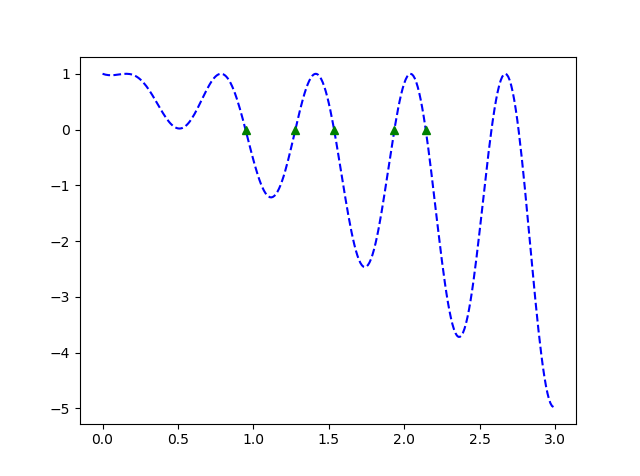
\includegraphics[width=3in]{BisectionPlot.png}} \\
    \subfloat[Section Method]{\label{fig:bisec}\includegraphics[width=3in]{SecantPlot.png}}
    \subfloat[Riddler's Method]{\label{fig:bisec}\includegraphics[width=3in]{RiddlersPlot.png}}
    \caption{Approximation Plots for Three Root Finding Methods}
    \label{VVP}
\end{figure}

\begin{figure}
    \centering
    \includegraphics[width=3in]{TotalErrorPlot.png}
    \caption{Error Values for each method per Iteration}
    \label{fig:error}
\end{figure}

\end{document}
